\subsection{Canal Reto}

Para o caso onde a artéria coronária não possui aterosclerose,
podemos modelar o problema como um escoamento entre placas retas e paralelas
como é feito no caso do \textit{Escoamento de Poiseuille}.
A Fig. \ref{velocity evolution straight} apresenta o perfil
de velocidade transiente ao longo da coordenada $y$ no
meio do canal ($x=5R$). 

\begin{figure}[H]
     \centering
     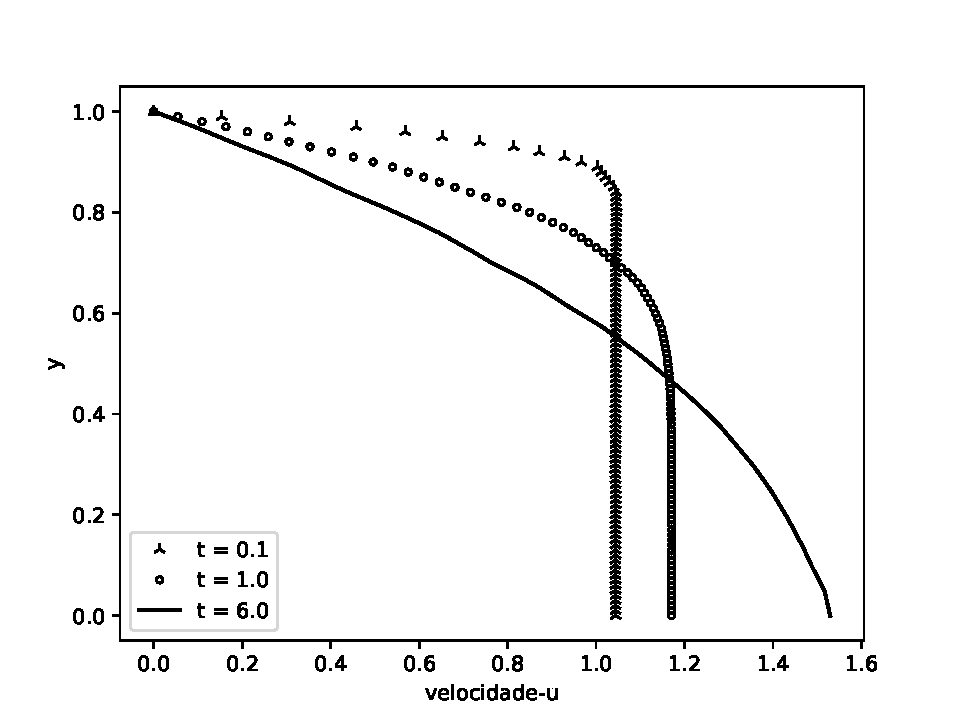
\includegraphics[scale=1]{cap_solution/figure/vel_Straight_evol.pdf}\\
     \caption{Evolução no tempo do perfil da velocidade para o Canal Reto.}
     \label{velocity evolution straight}
\end{figure}

\medskip
A Fig. \ref{velocity field straight} apresenta a evolução no tempo e no espaço
do campo de velocidade para a metade do domínio já que os resultados são simétricos
na direção $y$. O campo de velocidade é representado com os valores adimensionais
onde a cor vermelha se refere ao valor $u=1.5$ e a cor azul $u=0$. Transformando em
valores dimensionais temos $u=18cm/s$ e $u=0cm/s$ respectivamente.
 
\begin{figure}[H]
     \begin{minipage}{.50\linewidth}
      \centering
      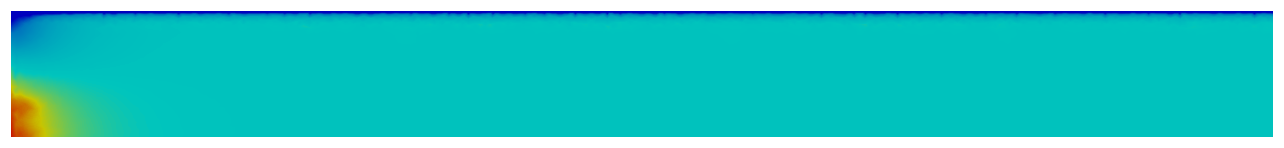
\includegraphics[scale=0.17]{cap_solution/figure/vel_Straight20.png}\\
      t = 0.1
     \end{minipage}%
     \begin{minipage}{.50\linewidth}
      \centering
      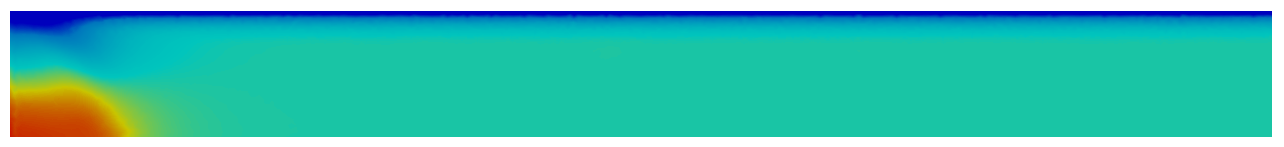
\includegraphics[scale=0.17]{cap_solution/figure/vel_Straight100.png}\\
      t = 0.5
     \end{minipage}
     \begin{minipage}{.50\linewidth}
     \medskip
      \centering
      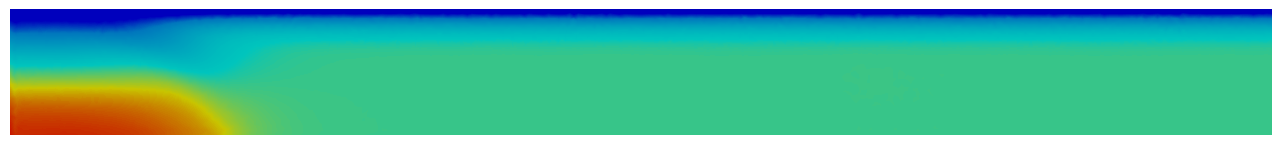
\includegraphics[scale=0.17]{cap_solution/figure/vel_Straight200.png}\\
      t = 1.0
     \end{minipage}%
     \begin{minipage}{.50\linewidth}
     \medskip
      \centering
      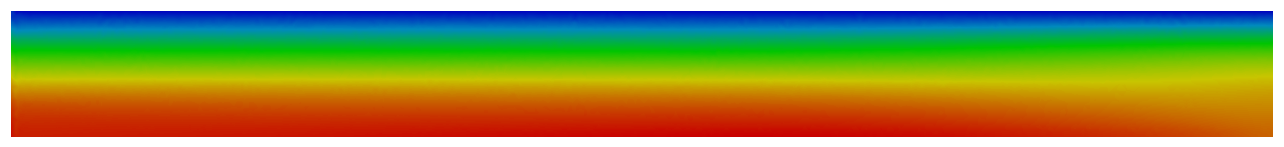
\includegraphics[scale=0.17]{cap_solution/figure/vel_Straight1200.png}\\
      t = 6.0
     \end{minipage}
     \medskip
     \caption{Evolução no tempo e no espaço do campo de velocidade para o Canal Reto.}
     \label{velocity field straight}
\end{figure}

